\part{Architekturen}
\section{Strukturierung komplexer Systeme}
\textbf{Nennen Sie zwei mögliche Konzepte zur Strukturierung komplexer Systeme}
\begin{itemize}
    \item Hierachie
    \item Verhalten
\end{itemize}

\section{Funktionale Systemarchitektur}
\textbf{Welche potentiellen Vorteile bietet die Verwendung einer funktionalen Systemarchitektur}
\begin{itemize}
    \item Disskution der Systemstruktur unabhängig von der Hardware(Hardware können sich häufig ändern)
    \item Hardware-unabhangige Schnittstellenanalyse
    \item Ableitung der Hardware-Topologie aus den funktionalen Anforderungen $\rightarrow$ Hardware-Topologie richtet sich nach den funktionalen Anforderungen
    \item Hierarchie der Beschreibungsebenen als strukturierendes Element
\end{itemize}

\section{Hierarchische Mehrebenensysteme}
\textbf{Was zeichnet hierarchische Mehrebenensysteme aus?}
\begin{figure}[H]
    \centering
    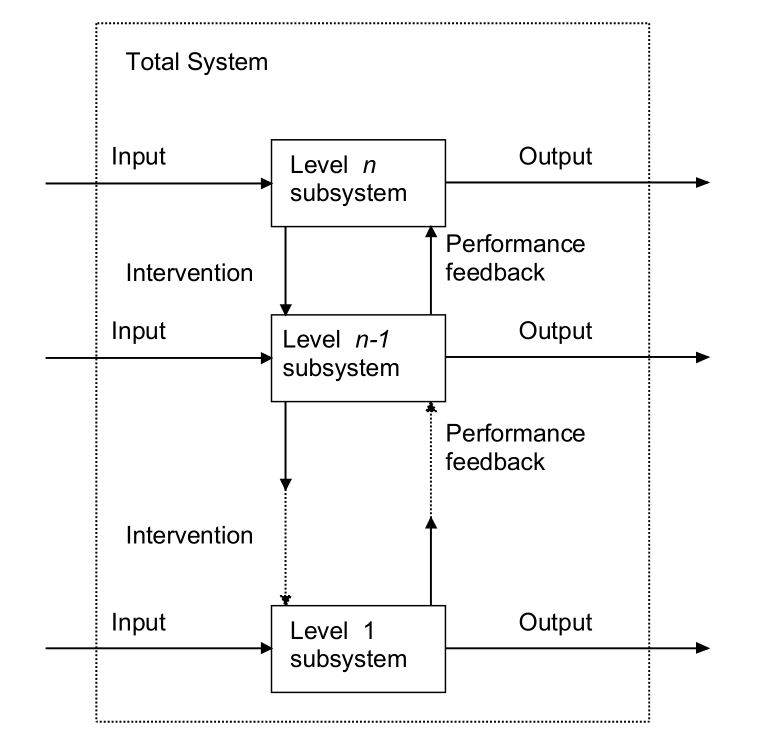
\includegraphics[width=.3\linewidth]{Graphics/hierarchie_mehrebenensystem.png}
    \caption{hierarchie Mehrebenensystem}
\end{figure}

\section{Verhaltensbasierte Architekturen}
\textbf{Was zeichnet  aus?}

bekanntester Vertreter: Subsumptionsarchitektur (Brooks, 1986)
(engl. subsume: zusammenfassen, unterordnen)
\begin{figure}[H]
    \centering
    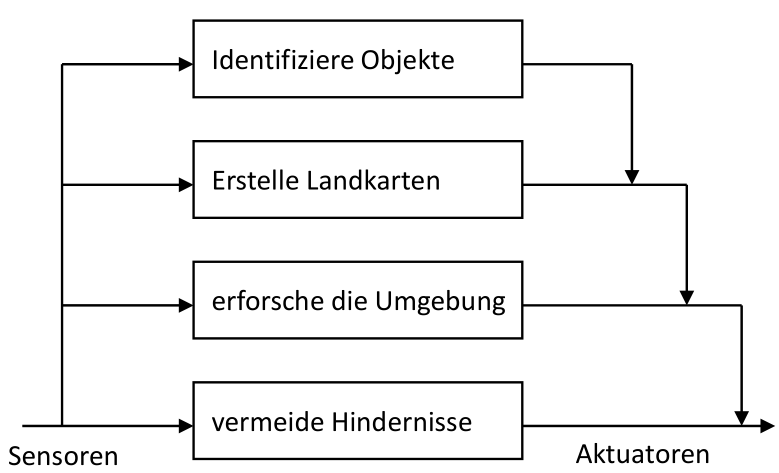
\includegraphics[width=.3\linewidth]{Graphics/subsumptionsarchitektur.png}
\end{figure}

\section{Drei-Ebenen-Modell nach Rasmussen}
\textbf{In welche drei unterschiedlichen Verhaltensebenen gliedert sich das Drei-Ebenen-Modells nach Rasmussen? Was zeichnet die Ebenen jeweils aus?}

\begin{itemize}
    \item Wissensbasiertes Verhalten
    \item Regelbasiertes Verhalten
    \item Fertigkeitsbasiertes Verhalten
\end{itemize}
\begin{figure}[H]
    \centering
    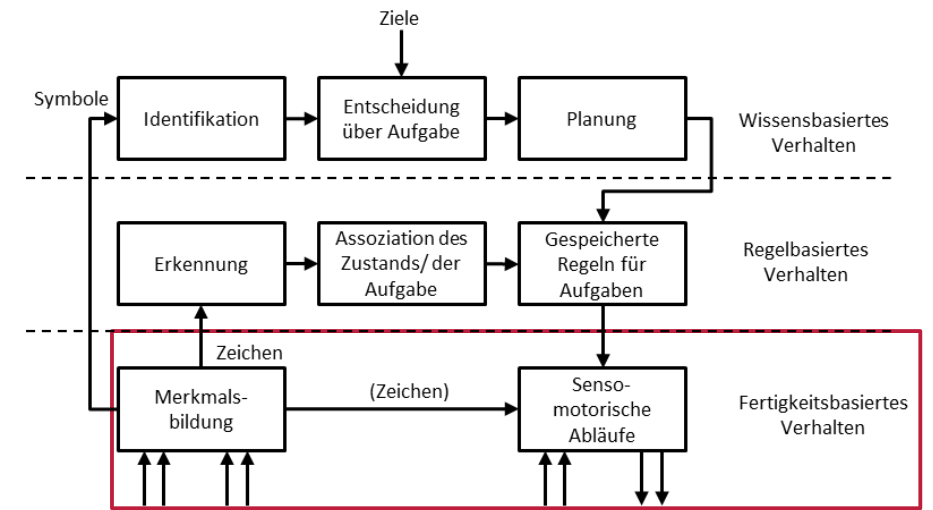
\includegraphics[width=.6\linewidth]{Graphics/Rasmussens_Drei_Ebenen_Medell.png}
    \caption{Rasmussens Drei-Ebenen-Modell}
\end{figure}